\clearpage
\section{Installation Sprach Assistant} \label{sec:Assistant}
Homeassitant ist die Schnittstelle, welche den Google Assitent mit Openhab verbindet. Die Kommunikation zwischen Homeassistant und Openhab findet über MQTT statt. Die Homeassistant Software wird auf ein weiteres Rasberrypi installiert.

\begin{enumerate}
	\item Download des Images für die Installation auf dem eigenen Raspi von der offiziellen Home Assistant \cite{assistant_installing_nodate}.
\item Micro SD Card flasen mit balenaEtcher \cite{noauthor_balenaetcher_nodate}. 
\item Mit ein USB Stick mit FAT32 formatieren und ihn als CONFIG benennen, ein Ordner mit dem Namen "network" erstellen, darin eine Text Datei erstellen, in der die Wlan Konfigurationen enthalten sind wie als Beipiel \cite{noauthor_home-assistantoperating-system_nodate} beschrieben oder in der Dokumentation enthalten.
\item USB Stick in und Micro SD Card mit Raspi verbinden und in Betrieb nehmen, dauert ca 20 min. Der USB Stick ist nur bei der ersten Inbetriebnahme notwendig.
\item Durch anwählen des Benutzernamen öffnet sich das Profil, Erweiterter Modus wählen.
\item Menupunkt Supervisor anwählen und in Add-on store File editor installieren, Start on boot und show in sidebar wählen
\item Mit File Editor Datei /config/configurationen.yaml bearbeiten: Mqtt-Message publish ermöglichen durch hinzufügen von Broker IP-Adresse und Port, siehe nachfolgende Abbildung.
\item Hinzu fügen von Schalter, welche mit Sprachbefehl Mqtt-Message generieren. Der Name des Schalters ist ebenso die Bezeichnung für den Sprachbefehl.
   \begin{figure}[H]
	\centering
	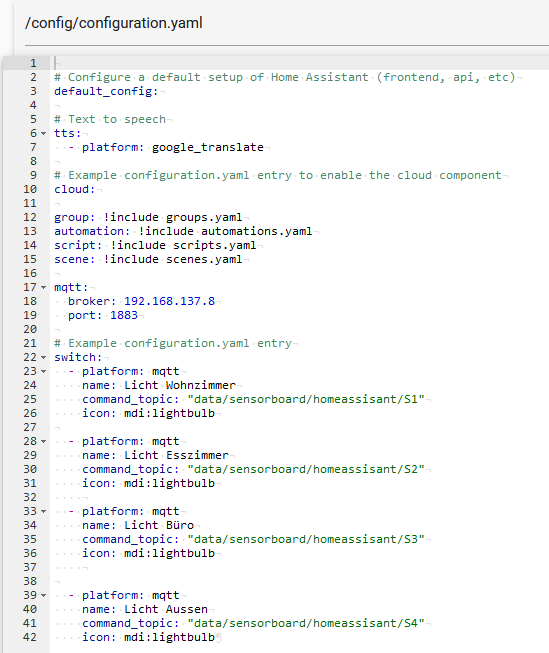
\includegraphics[width=0.75\textwidth]{graphics/Homeassostantconfig.PNG}
	\caption{Configfile Home Assistant} 	
	\label{pic: Configfile Home Assistant}
\end{figure}


 
\end{enumerate}

\subsection{Topics}
In Nachfolgenden Tabelle sind die generierten Topics, welche weiter in Openhab verwendet werden.
\begin{table}[H]
	\centering
	\begin{tabular}{|l|l|}
		\hline 
		Topic  & Funktion  \\ 
		\hline 
	data/sensorboard/homeassisant/S1 & Sprachbefehl von Google Assistant empfangen  \\ 
		\hline
	data/sensorboard/homeassisant/S2 & Sprachbefehl von Google Assistant empfangen \\ 
		\hline
	data/sensorboard/homeassisant/S3 & Sprachbefehl von Google Assistant empfangen \\ 
		\hline
		data/sensorboard/homeassisant/S4 & Sprachbefehl von Google Assistant empfangen  \\ 
		\hline
	\end{tabular} 	
	\label{tab: MQTT-Topics Home Assistant}
	\caption{MQTT-Topics Home Assistant}
\end{table}